% vim: ai sw=2

\documentclass[xcolor=dvipsnames,handout]{beamer}

\let\Oldemph\emph
\renewcommand{\emph}[1]{\textcolor{blue}{\Oldemph{#1}}}
\newcommand{\heading}[1]{\textbf{\textcolor{BurntOrange}{#1}}}
\newcommand{\header}[1]{\textbf{\texttt{\textcolor{WildStrawberry}{#1}}}}
\newcommand{\doc}[1]{\textbf{\texttt{\textcolor{OliveGreen}{#1}}}}

% Copyright 2004 by Till Tantau <tantau@users.sourceforge.net>.
%
% In principle, this file can be redistributed and/or modified under
% the terms of the GNU Public License, version 2.
%
% However, this file is supposed to be a template to be modified
% for your own needs. For this reason, if you use this file as a
% template and not specifically distribute it as part of a another
% package/program, I grant the extra permission to freely copy and
% modify this file as you see fit and even to delete this copyright
% notice.


\mode<presentation>
{
%  \usetheme{Warsaw}
\usetheme{Madrid}

  \setbeamercovered{transparent}
}

\usepackage[czech]{babel}
\usepackage[utf8]{inputenc}
\usepackage{times}
\usepackage[IL2]{fontenc}

\usepackage{graphicx}
\usepackage[final]{listings}
\usepackage{multirow}

\lstset{tabsize=2,numbers=none,showstringspaces=false,breaklines=true,
	breakatwhitespace=true,escapeinside={(*@}{@*)},
	basicstyle=\scriptsize,keywordstyle=\bfseries\color{OliveGreen},
	commentstyle=\color{blue}}

\title[PB173/01] % (optional, use only with long paper titles)
{PB173 -- Ovladače jádra -- Linux}

\subtitle{X. b.}

\author[J. Slabý]{Jiří~Slabý}

\institute[ITI] % (optional, but mostly needed)
{ITI, Fakulta Informatiky}

\date{30. 11. 2010}

\subject{}
% This is only inserted into the PDF information catalog. Can be left
% out.



% If you have a file called "university-logo-filename.xxx", where xxx
% is a graphic format that can be processed by latex or pdflatex,
% resp., then you can add a logo as follows:

% \pgfdeclareimage[height=0.5cm]{university-logo}{university-logo-filename}
% \logo{\pgfuseimage{university-logo}}



% Delete this, if you do not want the table of contents to pop up at
% the beginning of each subsection:
% \AtBeginSubsection[]
% {
%   \begin{frame}<beamer>
%     \frametitle{Outline}
%     \tableofcontents[currentsection,currentsubsection]
%   \end{frame}
% }


% If you wish to uncover everything in a step-wise fashion, uncomment
% the following command:

%\beamerdefaultoverlayspecification{<+->}

\begin{document}

\begin{frame}
  \titlepage
\end{frame}

%%%%%%%%%%%%%%%%%%%%%%%

\begin{frame}
  \frametitle{Systematické testování}

  \heading{Hledání chyb}
  \begin{itemize}
  \item Online
  \begin{itemize}
  \item Testování jádra
  \end{itemize}
  \item Offline
  \begin{itemize}
  \item Statická kontrola
  \item Model-checking
  \end{itemize}
  \end{itemize}

\end{frame}

\begin{frame}
  \frametitle{Testování jádra}

  \heading{Online (jádro musí běžet)}
  \begin{itemize}
  \item Automatické testy
  \begin{itemize}
  \item Kompilace různých konfigurací jádra
  \item Bootování systému
  \item \url{http://kisskb.ellerman.id.au/kisskb/branch/9/}
  \end{itemize}
  \pause
  \item Unit-testy
  \begin{itemize}
  \item Linux Test Project (LTP)
  \item Pomocí systémových volání se zkouší co nejvíce cest v ovladači
    \begin{itemize}
    \item Všechny \texttt{ioctl} s různými argumenty
    \item Nesprávné čtení přes \texttt{read} atp.
    \end{itemize}
  \item Domácí úkol
  \end{itemize}
  \end{itemize}

\end{frame}

\begin{frame}[fragile]
  \frametitle{Statická analýza I.}

  \heading{Jednoduchá analýza toku -- offline (stačí kód)}
  \begin{itemize}
  \item Relativně rychlá, mnoho falešných hlášení (FP)
  \item Existují (drahé \$) nástroje s minimem FP
  \item Mnoho nástrojů
  \begin{itemize}
  \item \textsc{Sparse}, \textsc{Smatch}, \textsc{Coverity},
    \textsc{Stanse} (ITI)
  \end{itemize}
  \end{itemize}

  \begin{table}
  \begin{tabular}{ccccccc}
  \begin{lstlisting}[language=C]
lock();
if (X)
  return;
unlock();
  \end{lstlisting} & $\Rightarrow$ &
  \parbox[c]{2.8cm}{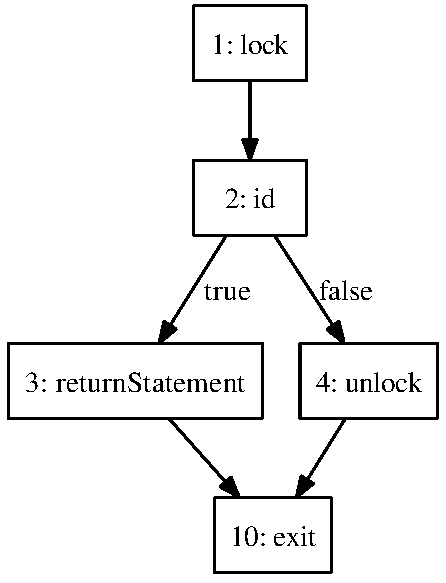
\includegraphics[width=3cm]{cfg}} & + &
  \parbox[c]{2.5cm}{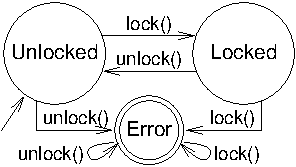
\includegraphics[width=2.5cm]{automaton}} & = &
  \parbox[c]{1.3cm}{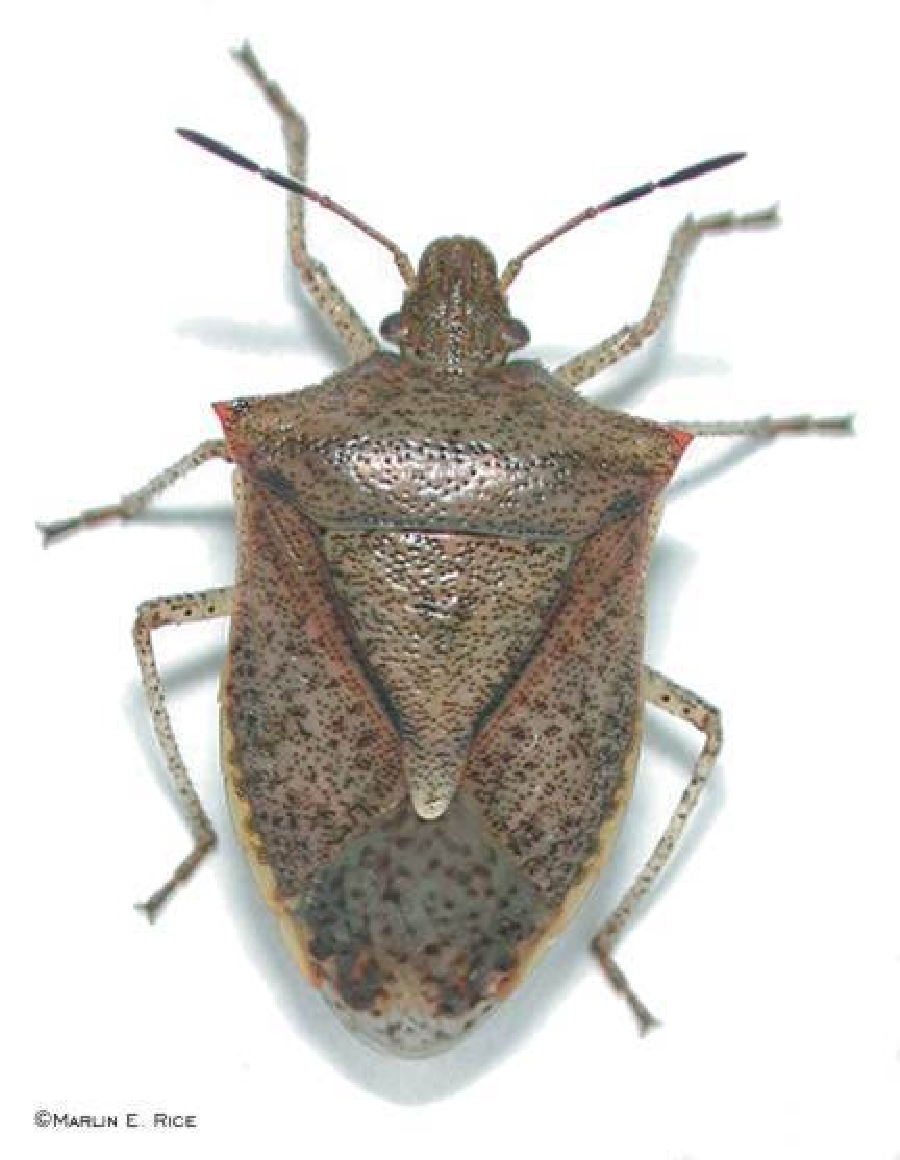
\includegraphics[width=1.3cm]{bug}} \\
  \scriptsize{Zdroj} & & \scriptsize{CFG} & & \scriptsize{Automat} & &
  \scriptsize{Chyby}
  \end{tabular}
  \caption{Postup základní statické analýzy}
  \end{table}

\end{frame}

\begin{frame}
  \frametitle{Úkol}

  \heading{Použití \textsc{Sparse} na pb173/10}
  \begin{enumerate}
  \item \texttt{make C=2}
  \item Opravit nahlášené chyby
  \end{enumerate}

\end{frame}

\begin{frame}[fragile]
  \frametitle{Statická analýza II.}

  \heading{Symbolická exekuce -- offline}
  \begin{itemize}
  \item Pomalejší (někdy výrazně), minimum FP
  \item Jen pár nástrojů
  \begin{itemize}
  \item \textsc{Klee} (kontroloval vybrané souborové systémy)
  \end{itemize}
  \end{itemize}

  \begin{table}
  \begin{tabular}{ccccccc}
  \begin{lstlisting}[language=C]
a /= b;
return a;
  \end{lstlisting} & $\Rightarrow$ &
  \begin{lstlisting}[language=XML]
%0 = sdiv %a, %b
ret %0
  \end{lstlisting} & + &
  \parbox[c]{2cm}{
    \begin{center}
    $(\varphi \wedge b = 0)$ \\
    $\vee$ \\
    $(\psi \wedge b \neq 0)$ \\
    $\Downarrow$ \\
    $b = 0?$
    \end{center}
  } & = &
  \parbox[c]{1.3cm}{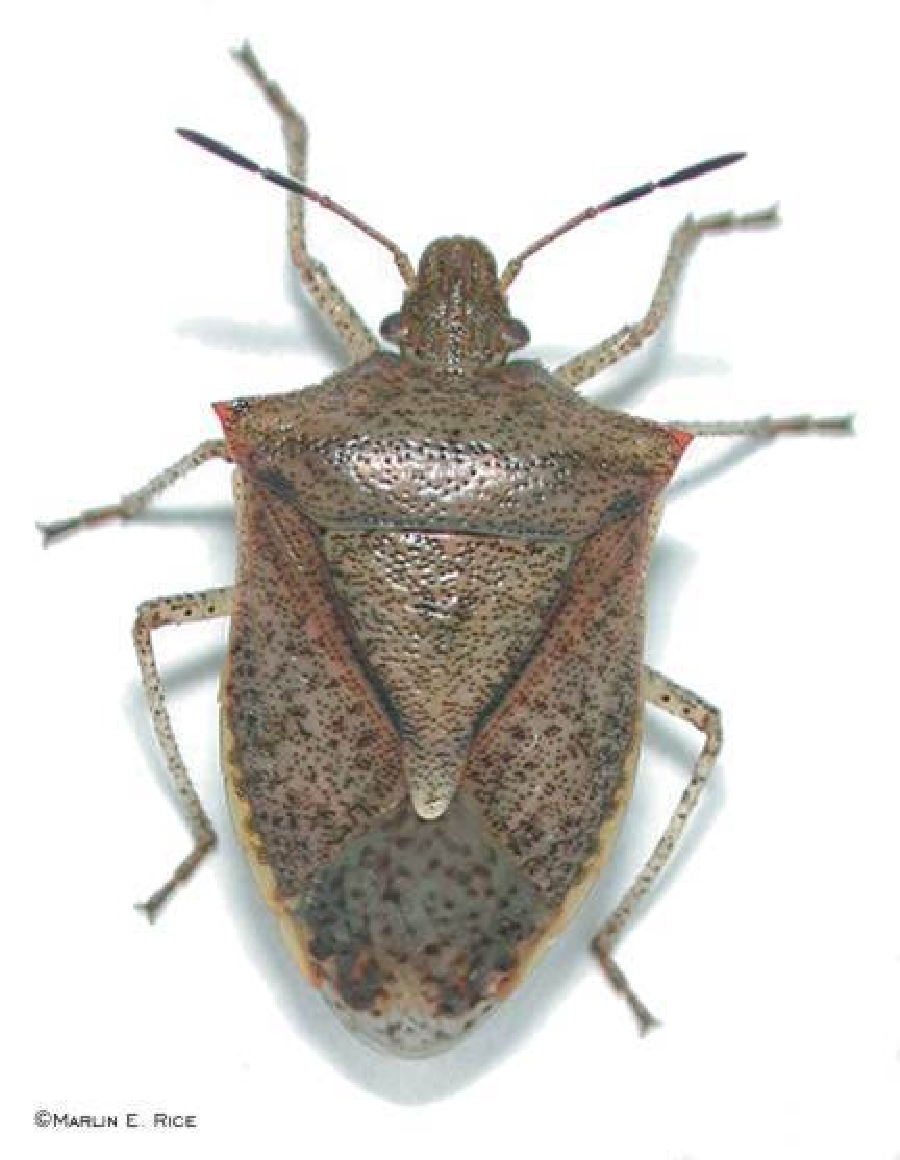
\includegraphics[width=1.3cm]{bug}} \\
  \scriptsize{Zdroj} & & \scriptsize{Low-level kód} & & \scriptsize{Řešení
  podmínky} & & \scriptsize{Chyby} \\
  & & & & \scriptsize{cesty} & &
  \end{tabular}
  \caption{Postup rozšířené statické analýzy}
  \end{table}

\end{frame}

\begin{frame}
  \frametitle{Model-checking}

  \heading{Offline}
  \begin{itemize}
  \item Matematicky se dokazuje, co může nastat a co ne
  \item Trpí explozí cest
  \item Jen pár nástrojů
  \begin{itemize}
  \item \textsc{Spin}
  \end{itemize}
  \item \emph{Vstup}: model chování, kód
  \item \emph{Výstup}: za jakých podmínek je model splněn
  \end{itemize}

\end{frame}

\begin{frame}
  \frametitle{Další témata}

  \begin{itemize}
  \item S/G DMA, MSI či jiné HW chuťovky
  \begin{itemize}
  \item Nemáme HW, pouze teoreticky
  \end{itemize}
  \item Základy HW (paging, KBD, VGA/VESA, PIC, TIMER, PCI BIOS)
  \begin{itemize}
  \item Spustit qemu bez OS a pracovat s (emulovaným) HW
  \end{itemize}
  \item Opravdové ladění chyb
  \begin{itemize}
  \item Odladit kód s úmýslně přidanými chybami
  \item K dispozici bude Oops
  \end{itemize}
  \item Síťovky (network stack)
  \begin{itemize}
  \item Vyrobit virtuální síťovku
  \end{itemize}
  \item Opakování jakéhokoliv tématu ze cvičení
  \begin{itemize}
  \item Např. víc do hloubky
  \end{itemize}
  \item Práce s GITem
  \item Perf
  \item \ldots
  \end{itemize}

\end{frame}

\end{document}

